\documentclass[conference,letterpaper,onecolumn]{IEEEtran}

\usepackage{graphicx}
\usepackage{psfrag}
\usepackage{stfloats}
\usepackage{epsfig}
\usepackage{pifont}
\usepackage{amssymb}
\usepackage{fixltx2e}
\usepackage{amsmath}
\usepackage{rotate}
\usepackage{anysize}
\usepackage{float}
\usepackage{fancybox}
\usepackage{subfig}

\newcommand{\pig}[1]{\mbox{\boldmath ${#1}$}	}

\newtheorem{Theod}{{\bf Definici\'on}}

\setlength{\oddsidemargin}{5mm}
\setlength{\evensidemargin}{5mm}
\setlength{\topmargin}{4mm}
\setlength{\textwidth}{15cm}
\setlength{\columnsep}{5mm}
\setlength{\textheight}{24cm}

\begin{document}

\title{Bounded Homotopy with four solution lines applied to nonlinear circuit simulation}

\author{\authorblockN{H\'ector V\'azquez-Leal}
\authorblockA{Universidad Veracruzana\\
Facultad de Instrumentaci\'on Electr\'onica\\
Xalapa, Veracruz, M\'exico\\
Email: hvazquez@uv.mx}
\and
\authorblockN{Luis Hern\'andez-Mart\'{\i}nez}
\authorblockA{INAOE\\
Departamento de Electr\'onica\\
Email: luish@inaoep.mx}
\and
\authorblockN{Arturo Sarmiento-Reyes}
\authorblockA{INAOE\\
Departamento de Electr\'onica\\
Email: jarocho@inaoep.mx}
\and
\authorblockN{Roberto Casta\~neda Sheissa}
\authorblockA{Universidad Veracruzana\\
Facultad de Instrumentaci\'on Electr\'onica\\
Xalapa, Veracruz, M\'exico\\
Email: rocastaneda@uv.mx}
}

\maketitle

\begin{abstract}

This work shows a new double bounded Homotopy based on a polynomial formulation with four lines separated by a fixed distance. The new Homotopy scheme presents a bounding between the two internal solution lines and the symmetry axis, which allows to establish a stop criterion for the simulation. Besides, the initial and final points on this new double bounded Homotopy can be set arbitrarily. New mathematical properties fo the new Homotopy will be introduced and be exemplified by means of some mathematical and circuital cases.
\end{abstract}
 
\section{Introduction}

The electronic industry, so demanding and competitive as well, constantly pushes circuit's area to the limit of the human knowledge. This has created an accelerated growing on the integration leves for the integrated circuits (IC). In \cite{lmoore} Moore's Law is introduced which describes the exponential growing on the integrated circuits density, reaching the 2 billion transistors within a single integrated circuit in 2008. Thus the need to develop software tools to simulate the circuit performance that every day is becoming more complex. In particular, the Homotopy has direct impact in simulation tools for ICs, and in general into any science area where a phenomenon can be modelled using non-linea equation systems. The reason that one given circuit could have more than one operating point in DC and the way to solve such points are solved using Homotpy methods \cite{homo_ogrodzki}.

The task to find the DC solution is important because this analysis is the starting point fot the rest of the common test regularly done through the circuit design process (for instance, small-signal analysis). This analysis consists in finding the solutions for a non-linear equation system (NAEs) from the ICs \cite{Schwa_book,mnaxx}. These NAEs becomes complex due to the accelerated increase of the transistores employed in the IC and by the use of complex models used (as a result of reducing the components dimensions) causing two phenomena: existence of multiple unexpected operating points and convergence failures for the Newton-Raphson (NR) method). The NR method is employed by the majority of the integrated circuit simulators. The reason for the widespread use of the Newton method is its quadratic convergence rate which reduce the computing times for the simulations. Nevertheless, the Newton method suffers some  convergence issues \cite{cont_quasi,Schwa_book} which are described by cases in figure \ref{NRG} where $f(x)$ is the equation to be solved.

\begin{itemize}
\item {\bf Case $A$}  Can be observed how the method converge to a single solution. This method is locally convergent \cite{Schwa_book} because if the initial point es not close enough to the solution, the method could fail.
\item {\bf Case $B$} In this case the method oscillates in certain region because is based in a functioning principle based in curve tangents for the $f(x)$ curve. It also shows how the initial point selection can affect, radically, the method´'s convergence. The oscillation is produced by an undetermined arbitrarily number of iterations set to limit each simulation, once this number is reached the simulation is stopped throwing a convergence error; this situation serves the base to use alternative methods to find solutions.
\item {\bf Case $C$} Here can be seen the way the method converges to another solution.The choice to select a different initial point may lead to locate another solution but this method is unable to locate more than one solution by simulation. 
\item {\bf Case  $D$} This case diverges given its functioning nature based on tangents to the cruve $f(x)$. The divergence produces high values on variables which can be translated in  numerical overflow that cause failures and simulation to be finalized.
\end{itemize}

%%FIGURA
\begin{figure}[hbtp]
\centering
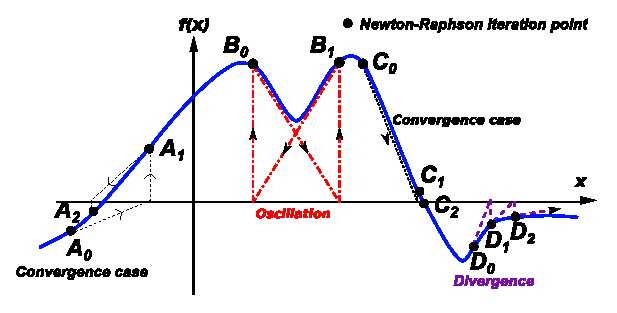
\includegraphics[scale=1.3]{figs/divergencia.eps}
\caption{Newton-Raphson convergence and divergence cases.}
\label{NRG}
\end{figure}

Convergence problems (cases $B$ and $D$ ) for the NR method becomes more difficult as the complexity of equations increase due by the high non-linearities present. In fact, the NR method was used since the development for the first integrated circuit simulator SPICE \cite{homo_hspice} in 1975, by that time the densest circuits included about 10,000 transistor by IC, which notoriously contrasts with the more than 2 billion transistors \cite{lmoore} that a modern IC can contain; this is a huge growth on size and complexity for the problem to be solved by Newton's method. Besides to the increase on the number of transistors, the complexity of the  physical models which describe the behavior of current transistors (because being of sub-micron dimensions means more complex physical behaviors \cite{homo_BSIM}).

The ERDD circuit in figure \ref{2tunelx} contains the following series setting: two tunnel diodes (K3 and K4), one resistor (R2), and a voltage source (V1).
 
\begin{figure}[hbtp]
\centerline{
\epsfxsize=70mm 
\epsffile{chap4/figs/erdd.eps}
}
\caption{Two tunnel diodes circuit.}
\label{2tunelx}  
\end{figure}

Both tunnel diodes are identical showing the following branch function:

\begin{displaymath}
i=I_p({V \over V_p})e^{1-{V \over V_p}}+I_0e^{{q \over {KT}} V}
\end{displaymath}

where the value for the voltage source $V_1$ is $1V$ and for resistor $R_2$ is $20\Omega$. Besides, both tunnel diodes ($K_3$ and $K_4$) have the same model with coefficients:
$Ip=100 \times 10^{-3}$,
$V_p=50 \times 10^{-3} $, $I_0=1\times 10^{-9}$ y ${q \over {KT}} = 40$. 

This circuit has a total of 9 operating points or solutions, from which integrated circuit simulators are capable to locate one solution, at best. The former can be exemplified using the simulator LTSpice IV \cite{LTSpice} to perform a DC analysis for the circuit shown in figure 3. The chosen starting point is $v_1=v_2=v_3=v_4=2V$ for the NR method. The result is shown in figure \ref{newtonfail}, it is caused by a convergence failure on the NR method ({\sf Direct Newton iteration failed to find .op point}). This is a serious event for the NR method since the circuit contains just 4 transistors compared to commercial circuits that can contain millions or billions (this is a huge increase on the complexity of the equilibrium equation). Once the NR method fails, the simulator executes automatically a back-up numerical method called conductance staggering \cite{homo_spectre,homo_hspice,homo_aplac}, which finds one operating point. In fact, the conductance staggering is a primitive type of Homotopy classified as natural type Homotopy.

\begin{figure*}[tbp]
\centering
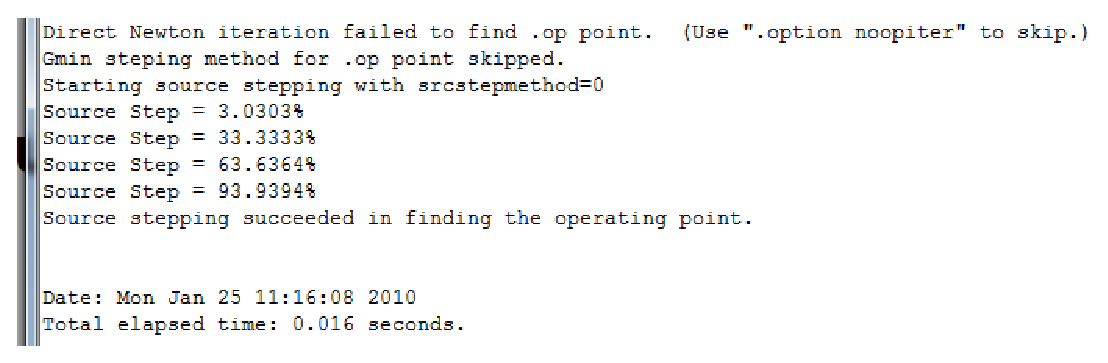
\includegraphics[width=15cm]{figs/newtonfail.eps}
\caption{Error message for the Newton-Raphson method in LTSPICE IV.}
\label{newtonfail}
\end{figure*}

Circuit designers face convergence failures commonly using the NR method and back-up methods, thus, as last resort, the modification of some parameters of the numerical engine are enforced expecting to reach convergence. This situation increase design times, making the entire design cycle slow and expensive. This situation, by itself, justifies the use of alternative methods to Newton like Homotopy to locate the operating point. Nevertheless, there are more reasons to use Homotopy methods like the existence of multiple operating points. This is because, unlike Newton, Homotopy is capable to locate multiple operating points. This is important because it is possible that the designer could approve certain DC operating point (found by the Newton method) that may not be physically present in the already fabricated IC. This is translated in malfunctioning of the circuit which could, in the end, represent high loses for the company in financial terms.

Homotopy methods \cite{BHLHOM,homo_ushida1,homo_green2,homo_DWolfMulti,homo_ArtificialP} have been proved as useful to locate multiple operating points and converge to solutions where the Newton method does not. Nevertheless, Homotopy methods are affected by certain inconveniences, among them are: stop criterion and computing time.

\section{Double bounded Homotopy}

Considering the existance of two solution lines, one at $\lambda=a$ and the other at $\lambda=b$ the Homotopy formulation is the following:

\begin{equation}
\pig{H}(\pig{f}(\pig{x}),\lambda ) =\pig{0}
\label{H2M}
\end{equation}

where $\lambda$ is the Homotopy variable and $\pig{H}^{-1}(\pig{0})$ the family of solutions that makes up the Homotopy path, such that:

\begin{itemize}
\item For $\lambda=0.5(a+b)$ the solution for $H^{-1}(.)$ is known
or easy to obtain, in computer terms. This point is known as the initial point for the Homotopy  ($\lambda_i$).
\item As for $\lambda=a$, $\pig{H}(\pig{f}(\pig{x}),\pig{a} )=\pig{f}(\pig{x})$.
Means that at $\lambda=a$ all solutions for $\pig{f}(\pig{x})$ are placed.
\item For $\lambda=b$, $\pig{H}(\pig{f}(\pig{x}),\pig{b} )=\pig{f}(\pig{x})$.
Means that at $\lambda=b$ all solutions for $\pig{f}(\pig{x})$ are placed.
\item The path for $\pig{H}^{-1}(\pig{0})$ is a continuous function for $\lambda$ in the range of  $a \leq \lambda \leq b $. 
\end{itemize}

\section{Double bounded polynomial Homotopy with four solution lines}

The double bounded polynomial Homotopy with 4 solution lines (DBP4) is defined by this equation:

\begin{equation}
{\small
\begin{array}{l}
\pig{H}(\pig{f}(\pig{x}),\lambda )=Q(x-x_i)(x-x_f) +C(\lambda-a/2)^2 \pig{f}(\pig{x})^2
\end{array}}
\label{homotopiaP}
\end{equation}

where {\small $Q=\lambda(\lambda+a)(\lambda-a)(\lambda-2a)$}, $a$ is a constant that represents separation between solution lines, $x_i$ is the initial point, $x_f$ the final point, and $C$ an arbitrary constant.

Based on the previous, Homotopy can be expressed in general way as:

\begin{displaymath}
\pig{H}(\pig{f}(\pig{x}),\lambda ) = \left\{\begin{array}{rl}
f(x^*)=0 & \textrm{for $\lambda=0$ y $x=x^*$}\\
(x-x_i)(x-x_f)=0 & \textrm{for $\lambda=a/2$}\\
f(x^*)=0 & \textrm{for $\lambda=a$ y $x=x^*$}
\end{array}\right.
\end{displaymath}

where $x^*$ is any solution for $f(x)$, $x_i$ and  $x_f$ are Homotopy's initial and final points, respectively.

This Homotopy contains 4 solution lines ($\lambda=-a$, $\lambda=0$, $\lambda=a$, and $\lambda=2a$). Nevertheless, the two solution lines for both ends are unconnected branches not used for tracing purposes. Squaring the function $f(x)$ has the finality to establish an even number of solutions (or operating points) which precisely produces the bounding and closes the Homotopy path inside the middle region.

\begin{figure*}[tbp]
{\tiny  
\centerline{
\psfrag{o}{$\lambda$}
\centering
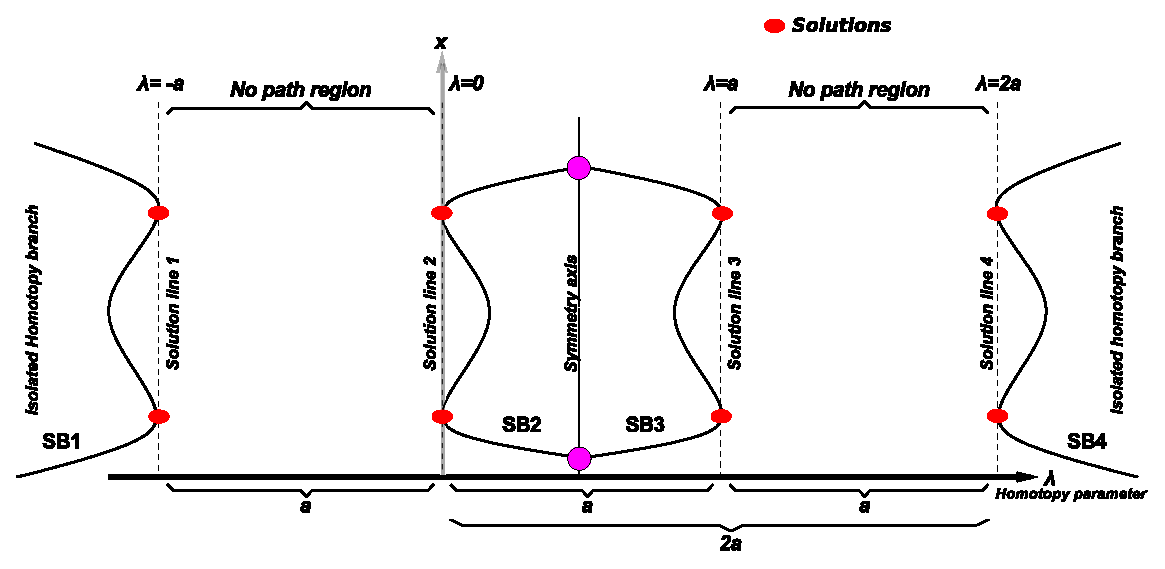
\includegraphics[width=14cm]{figs/doblelineapoli.eps}}}
\caption{General scheme for polynomial Homotopy with double solution.}
\label{doblehp}
\end{figure*}

Figure \ref{halftrack} shows how Homotopy path starts at $A=(x_i,a/2)$ on the symmetry axis, finds two roots (in region $SB3$) and finishes when a new crossing through the symmetry axis at $B=(x_f,a/2)$ is detected, which means that tracing for a symmetrical branch has been completed and fulfilling the stop criterion.

\begin{figure}[hbtp]
\psfrag{o}{$\lambda$}
\centering
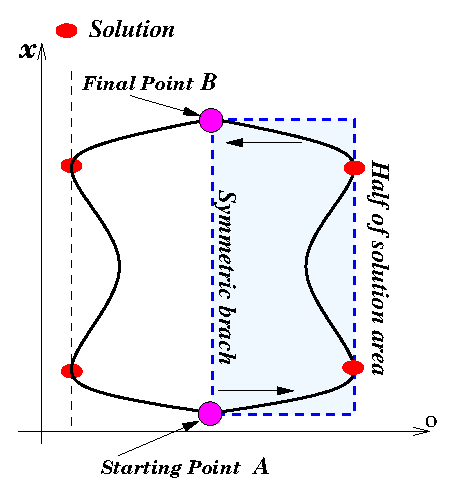
\includegraphics[scale=0.95]{figs/chap3/figs/dbh2.eps}
\caption{Stop criterion.}
\label{halftrack}
\end{figure}


The properties for this new Homotopy are presented in the following sub-sections:

\subsection{Symmetrical branches}

To obtain the branches for the Homotopy path, first the equation \ref{homotopiaP} is reformulated as follows:

\begin{equation}
{%\tiny
\begin{array}{l}
\pig{H}(\pig{f}(\pig{x}),\lambda )=\lambda(\lambda+a)(\lambda-a)(\lambda-2a)+(\lambda-a/2)^2 J(x)=0
\end{array}}
\label{homotopiaP1}
\end{equation}
where 
\begin{displaymath}
\begin{array}{l}
 J(x)= {Cf(x)^2 \over (x-x_i)(x-x_f)}
\end{array}
\end{displaymath}

Symmetrical branches shown in figure \ref{doblehp} can be derived solving $\lambda$ from equation \ref{homotopiaP1}. The result is 4 symmetrical branches. Each branch {\it SB1, SB2, SB3}, and {\it SB4} is linked to a different solution line $\lambda=[-a,0,a,2a]$, respectively. In order to trace the Homotopy path, the unconnected symmetrical paths {\it SB1} and {\it SB4} will be ignored because these open branches would make not possible to apply the stop criterion. Given the fact that {\it SB2} and {\it SB3} are connected and symmetrical, only one can be traced to obtain the full path and finalize the simulation. {\it SB3} is chosen as the tracing path, which touches obliquely the solution line $\lambda=a$.

\begin{table*}[tbp]
\center{ \large
\begin{tabular}{||c|c|c||}
\hline\hline
Symmetry branch  & Formulation  & Limit at $f(x^*)=0$   \\ \hline\hline \vspace{1mm}
{\it SB1} & $\lambda_1= {{a-\sqrt {5\,{a}^{2}+2\,\sqrt { \left( J \left( x \right) +4
\,{a}^{2} \right)  \left( J \left( x \right) +{a}^{2} \right) }+2\,J
 \left( x \right) }} \over {2}}$ & $\lambda=-a$ \\  \hline \vspace{1mm}
{\it SB2} & $\lambda_2= {{a-\sqrt {5\,{a}^{2}-2\,\sqrt { \left( J \left( x \right) +4
\,{a}^{2} \right)  \left( J \left( x \right) +{a}^{2} \right) }+2\,J
 \left( x \right) }} \over {2}}$  & $\lambda=0$ \\  \hline \vspace{1mm}
{\it SB3} & $\lambda_3= {{a+\sqrt {5\,{a}^{2}-2\,\sqrt { \left( J \left( x \right) +4
\,{a}^{2} \right)  \left( J \left( x \right) +{a}^{2} \right) }+2\,J
 \left( x \right) }} \over {2}}$ & $\lambda=a$ \\  \hline \vspace{1mm}
 {\it SB4} & $\lambda_4= {{a+\sqrt {5\,{a}^{2}+2\,\sqrt { \left( J \left( x \right) +4
\,{a}^{2} \right)  \left( J \left( x \right) +{a}^{2} \right) }+2\,J
 \left( x \right) }} \over {2}}$ & $\lambda=2a$ \\  \hline  \hline
\end{tabular}
}
\caption{Symmetrical branches}
\label{ramasx}
\end{table*} 


\subsection{Symmetry axis}

The symmetry axis is an important property for the double bounded Homotopy. In the particular case of the polynomial double bounded Homotopy the symmetry axis is:

\begin{equation}
\lambda_{sym}= {a \over 2}
\label{sym}
\end{equation}

This symettry axis belong to the symmetry relationship between $SB2$ and $SB3$ branches.

As shown in figure \ref{simetria}, this relationship must be fulfilled:

\begin{displaymath}
\lambda_3-\lambda_{sym}=\lambda_{sym} -\lambda_2
\end{displaymath}

Replacing the value for $\lambda_{sym}$, we obtain:

\begin{displaymath}
\lambda_3-0.5a=0.5a-\lambda_2
\end{displaymath}

Then, replacing $\lambda_2$ and $\lambda_3$ for their respective functions the next relationship is found:

\begin{displaymath}
\begin{array}{l}
0.5a+0.5\sqrt{G(\pig{x})}-0.5a= 0.5a-0.5a+0.5\sqrt{G(\pig{x})}
\end{array}
\end{displaymath}

where {\small $G(\pig{x})=\sqrt {5\,{a}^{2}-2\,\sqrt { \left( J \left( x \right) +4 \,{a}^{2} \right)  \left( J \left( x \right) +{a}^{2} \right)}} $

Reducing terms:
\begin{displaymath}
\begin{array}{c}
0.5\sqrt{G(\pig{x})}=0.5\sqrt{G(\pig{x})} \\
0=0
\end{array}
\end{displaymath}

The proof for this equality shows that the Homotopy path is symmetrical around the symmetry axis.

{
\tiny
\begin{figure}[hbtp]
\psfrag{o}{\tiny $\lambda$}
\psfrag{o1}{\tiny $\lambda_3$}
\psfrag{o2}{\tiny $\lambda_2$}
\psfrag{o3}{\tiny $\lambda_3-\lambda_{sym}$}
\psfrag{o4}{\tiny $\lambda_{sym}-\lambda_2$}
\centering
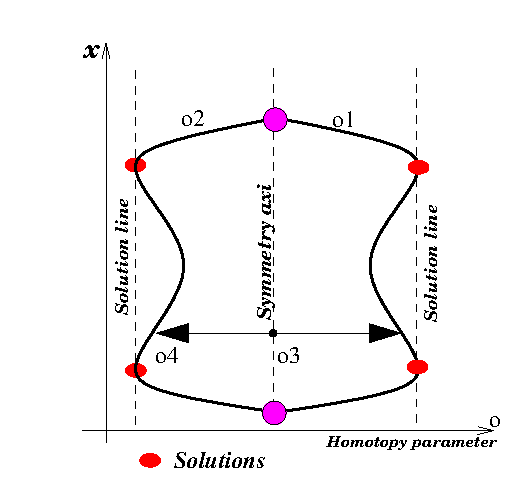
\includegraphics[width=9cm]{figs/simetria.eps}
\caption{Symmetry of the Homotopy path.}
\label{simetria}
\end{figure}
}

\subsection{Initial point and final point}

The point where the Homotopy path starts is located right on the symmetry axis, therefore $\lambda_i=a/2$. Thus, replacing $\lambda_i$ in equation \ref{homotopiaP} cancels the term that contains the equilibrium equation $f(x)$, achieving:

\begin{displaymath}
\begin{array}{r}
\pig{H}(\pig{f}(\pig{x}),\lambda_i )=(x-x_i)(x-x_f)=0  \\
\end{array}
\end{displaymath}

Therefore, the initial point $x_i$ and final point $x_f$ are chosen arbitrarily.

Solving for $\lambda$ in equation \ref{homotopiaP} the branch SB3 is:

{
%\tiny
\begin{displaymath}
\lambda_3= {\frac {Fa+\sqrt {5\,{F}^{2}{a}^{2}-2\,F\sqrt { 4\,{F}^{2}{a}^
{4}+5\,F \left( f \left( x \right)  \right) ^{2}{a}^{2}+ \left( f
 \left( x \right)  \right) ^{4}}+2\,F \left( f \left( x \right) 
 \right) ^{2}}}{2F}}
\end{displaymath}
}
where $F=(x-x_i)(x-x_f)$. Now, the following limits are calculated:

\begin{equation}
 \displaystyle\lim_{x \to{x_i}}{\lambda_3}=0.5a 
 \label{demos1}
\end{equation}

\begin{equation}
  \displaystyle\lim_{x \to{x_f}}{\lambda_3}=0.5a
 \label{demos2}
\end{equation}

Hence, when $x$ tends to the value for the initial point $x_i$ or final point $x_f$, the Homotopy parameter $\lambda$ tends to the symmetry axis at $\lambda=0.5a$.

\subsection{Circuital rendering}

The circuital rendering for the double bounded Homotopy can be derived solving $f(x)$ from the Homotopy expression in equation \ref{homotopiaP}. From former equation can be concluded that there are non-linear current sources ($K_1$, · · · ,$K_n$) connected to every node of the circuit, where $n$ is the number of nodes, and $I$ the number of constant voltage sources ($E$).

\begin{equation}
I_{K_i}={\lambda(\lambda+a)(\lambda-a)(\lambda-2a)(V_{xk}-V_{{xk}_i})(V_x-V_{xk_f}) \over (\lambda-a/2)^2}
\label{Ikn}
\end{equation}

where $k=[1,n]$,  $V_{xk}$ are the nodal voltages of the circuit, $V_{{xk}_i}$ and $V_{{xk}_f}$ are constant values related to the initial and final points for each variable $V_{xk}$ in the Homotopy. Finally, the circuital rendering of the Homotopy at the symmetry axis can be seen in figure \ref{circ1}.

\begin{figure*}[tbp]
\centering
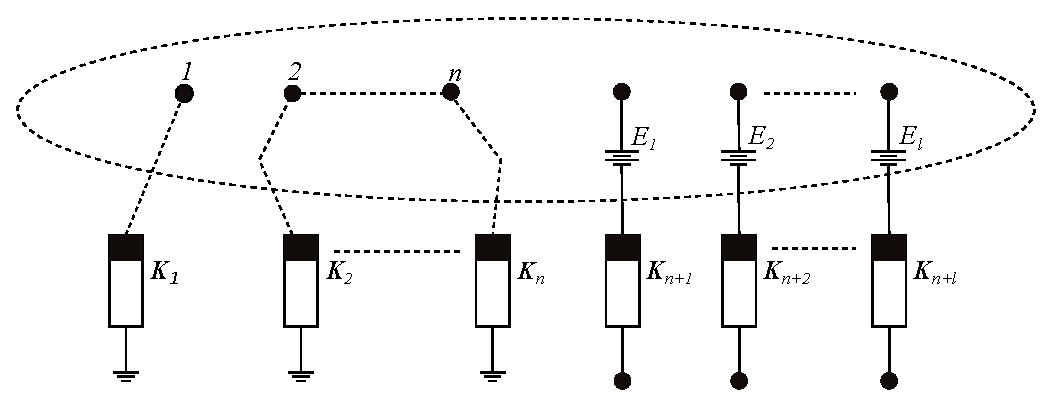
\includegraphics[scale=0.75]{figs/circ_1.eps}
\caption{Circuital rendering for the double bounded Homotopy.}
\label{circ1}
\end{figure*}

\subsection{Multiple variables}

When Homotopy is applied to a non-linear equation system with multiple variables, the generalization is given by:

\begin{displaymath}
\begin{array}{c}
H_1(f_1(x),\lambda)=Q(x_1-x_i)(x_1-x_f)+C(\lambda-a/2)^2f_1(x)^2 \vspace{5mm} \\
H_2(f_2(x),\lambda)=Q(x_2-x_i)(x_2-x_f)+C(\lambda-a/2)^2f_2(x)^2 \vspace{5mm} \\
H_3(f_3(x),\lambda)=Q(x_3-x_i)(x_3-x_f)+C(\lambda-a/2)^2f_3(x)^2 \\
\vdots  \hspace{30mm} \vdots  \hspace{30mm} \vdots \\
H_n(f_n(x),\lambda)=Q(x_n-x_i)(x_n-x_f)+C(\lambda-a/2)^2f_n(x)^2 \\
\end{array}
\end{displaymath}

where $n$ is the number of equations of the equilibrium equation $\pig{f}(\pig{x})$, $f_i$ represents every nodal equations or extra equations for non-NA compatible elements \cite{mnaxx}, $C$ is an arbitrary constant, and $Q=\lambda(\lambda+a)(\lambda-a)(\lambda-2a)$.

Figure \ref{poligono} presents a polygon showing in a descriptive way the behavior of the possible Homotopy paths staring from different initial points, result of combining the initial and final points for every $x$. Therefore, each vertex represents the possible start or ending for the Homotopy path. Next, some possible cases are described. The total number of vertexes for the polygon is $n^2$. 

\begin{itemize} 
\item In the case of point $p_1$ the Homotopy path ends at $p_5$, crossing through 3 operating points ($S_1$, $S_2$, y $S_3$).
\item For point $p_2$ the Homotopy path ends at $p_4$, crossing through 2 operating points ($S_2$ and $S_3$), which are common to the path described by $p_1-p_5$.
\item For the case of point $p_3$ the Homotopy path ends at $p_{(n^2)}$, crossing through 3 operating points ($S_1$, $S_2$, and $S_3$), which are common to the path described by $p_1-p_5$.
\end{itemize}

\begin{figure*}[tbp]
\centering
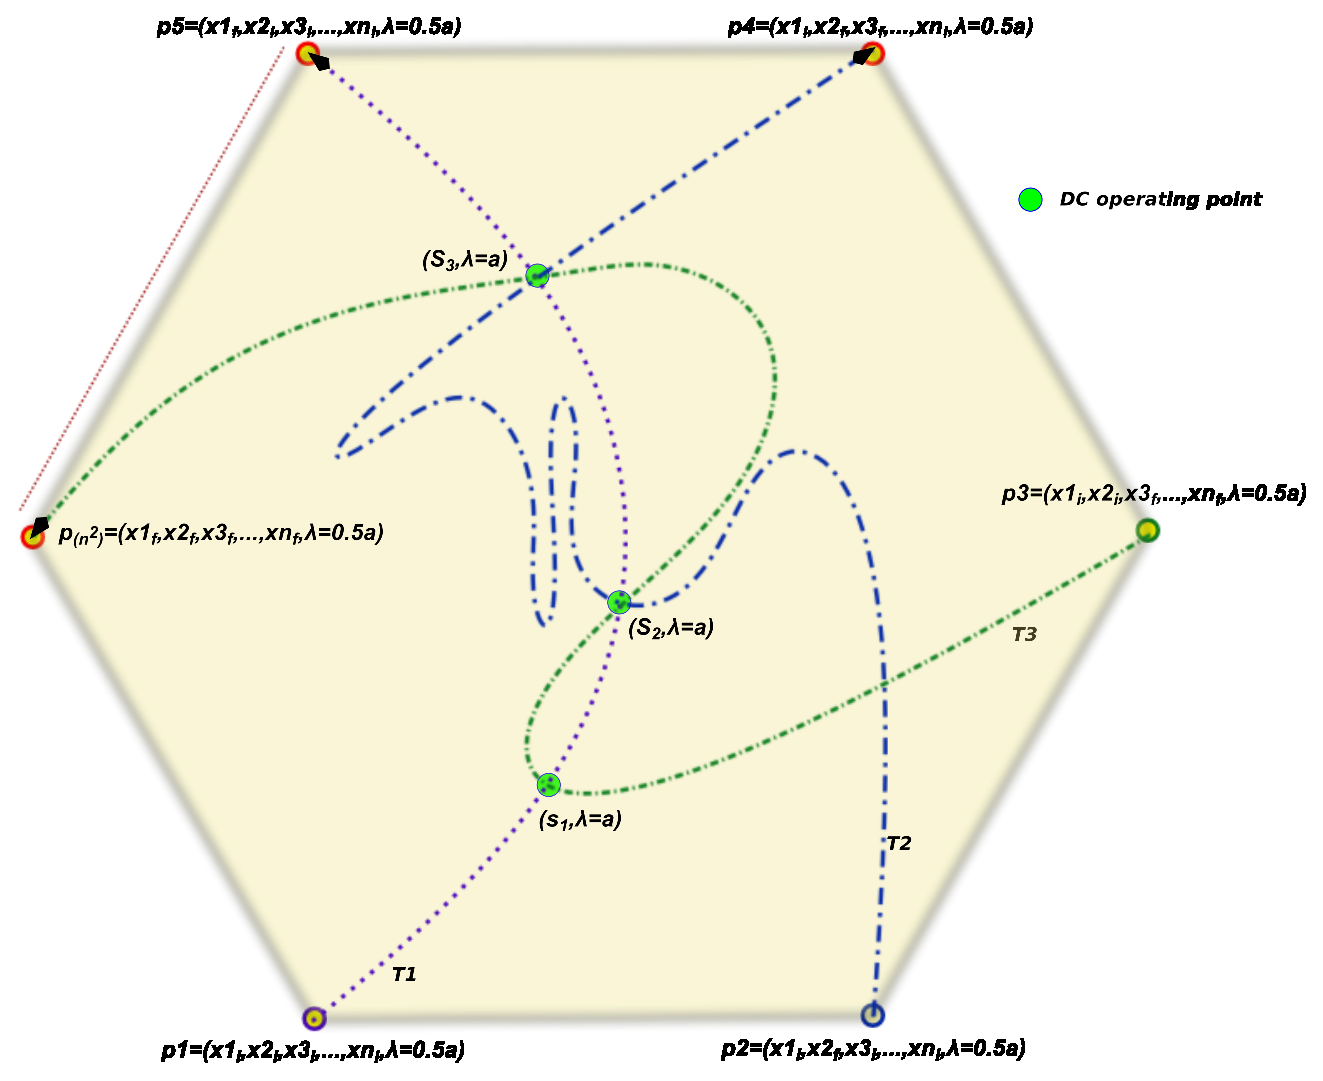
\includegraphics[scale=0.65]{figs/poligono.eps}
\caption{Initial and final points vertexes for the Homotopy path.}
\label{poligono}
\end{figure*}

\subsection{Curvature radius}

The curvature radius for the Homotopy path will be employed as an analysis tool {\it cualitativamente} of the paths on strategic points like solutions and turning points (see figure \ref{radio1}). Curvature radius for a curve in a point is the radius for a circle with curvature equivalent at that point of the curve.

The equation for the curvature radius is:

\begin{displaymath}
\rho=  \Bigg |{{(1 + (y')^2)^{3/2}} \over {y''}} \Bigg |
\end{displaymath}

where $y$ is a function $y(x)$, $y'$ is the first derivative of $y(x)$ with respect to $x$ and
$y''$ is the second derivative of $y(x)$ with respect to $x$. In terms of the Homotopy path, the first derivative $y'$ is equal to ${ {d \lambda} \over {dx}}$ and the second derivative $y''$ is equal to ${ {d^2 \lambda} \over {dx^2}}$.

\begin{figure}[hbtp]
\centering
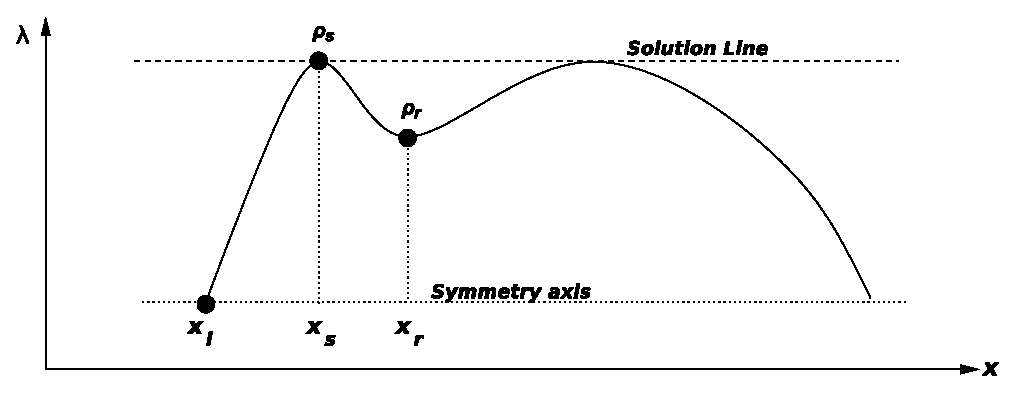
\includegraphics[scale=0.8]{figs/chap3/figs/radiob.eps}
\caption{Solution point $\rho_s$ and turning point $\rho_r$}
\label{radio1}
\end{figure}

The slope of the Homotopy path at the solution points and turning points is zero ($y'={ {d \lambda} \over {dx}} =0$), property that can be used to simpplify the expression for the curvature radius in those points, like:

\begin{displaymath}
\rho= \Bigg | {1 \over {{ {d^2 \lambda} \over {dx^2}}}} \Bigg |
\end{displaymath}

Now, $\lambda_3$ from equation SB3 in table \ref{ramasx} is derived twice with respect to $x$ and considering $a$ and $C$ as constants. Next, $f(x)$ is replaced by zero because it is the solution point, we obtain:

\begin{displaymath}
\rho_{s}=\left[4\,{\frac {a \left( x-x_i \right)  \left( x+x_f \right) }{  C
   \left( {\frac {d}{dx}}f \left( x \right) \right)^{2}}}\right]_{x=x_s}
\end{displaymath}

where $x_s$ is the value of the solution and $a$ represents the separation between solution lines.

The equation $\rho_{s}$ allows to conclude that distance $a$ between solution lines affects the sharpness of the Homotopy path on the solutions, in such a way that the curve is more acute as solution lines approach (each other) and flattens as solution lines distance each other. Besides, constant $C$ also affects the curve, flattening on the solution when$C$ increases and more acute as $C$ decreases.

The point where path returns to the solution search is called turning point $\rho_r$. The study of the curvature radius at the turning point $\rho_r$ complements with the study of the curvature radius at solutions $\rho_s$ in order have a deeper understanding of the qualitative behavior of the Homotopy path. At the turning point, the derivative of $\lambda$ with respect to $x$ equals zero. Besides, the turning point spatially matches the critical points of function $f(x)$, thus the derivative of $f(x)$ with respect to $x$ is zero.

In order to simplify the equation for the curvature radius it is assumed that:

\begin{displaymath}
\begin{array}{l}
 j(x)= {f(x)^2 \over (x-x_i)(x-x_f)}
\end{array}
\end{displaymath}

Therefore, the equation for the curvature radius is:

{
%\tiny
\begin{displaymath}
\rho_{r}=\left[{4\,\sqrt {5\,{a}^{2}- 2\,\sqrt {4\,{a}^{4}+ 5\,Cj \left( x
 \right) {a}^{2}+{C}^{2} \left( j \left( x \right)  \right) ^{2}}+ 2
\,Cj \left( x \right) } \over \left( -{\frac {5\,C \left( {\frac {d^{2}}{d{x
}^{2}}}j \left( x \right)  \right) {a}^{2}+2\,{C}^{2}j \left( x
 \right) {\frac {d^{2}}{d{x}^{2}}}j \left( x \right) }{\sqrt {4\,{a}^{
4}+5\,Cj \left( x \right) {a}^{2}+{C}^{2} \left( j \left( x \right) 
 \right) ^{2}}}}+2\,C{\frac {d^{2}}{d{x}^{2}}}j \left( x \right) 
 \right)} \right]_{x=x_r}
\end{displaymath}
}

where $x_r$ is the value for $x$ at the turning point.

To evaluate qualitatively the behavior of the curvature radius is necessary to carry out the following symbolic limits:

\begin{equation}
 \displaystyle\lim_{f(x) \to{+}\infty}{|\rho_{r}|}=\infty
 \label{rcurv1}
\end{equation}

\begin{equation}
 \displaystyle\lim_{f(x) \to{+}0}{|\rho_{r}|}= \left[8\,{\frac {a}{C{\frac {d^{2}}{d{x}^{2}}}f \left( x \right) }} \right]_{x=x_r} 
  \label{rcurv2}
\end{equation}

The limit for equation \ref{rcurv1} shows that when $f(x)$ tends to high values, the curvature radius grows, leaving the curve flat. When $f(x)$ has high values (evaluated at turning point $x_r$) is fairly common on the nodal equations of the circuit. Therefore, the Homotopy path will tend to stay close to the solution line $\lambda=a$. Suppose that a polynomial double bounded Homotopy is solved with $a=1$. In figure \ref{fig:xxx1}(a) is shown the symmetric branch located at the right corresponding to $\lambda=1$. In the latter figure is difficult to differentiate between solutions and turning points. Closing-up to the solution line at $\lambda=1$ (see figura \ref{fig:xxx1}(b)) allows to appreciate the solutions and turning points. This phenomenon was checked simulating various circuits and non-linear equations. The limit for equation \ref{rcurv2} indicates that when $f(x)$ tends to small values, the curvature radius es proportional to the value for solution line $a$ and inversely proportional to constant $C$.

\begin{figure}[hbtp]
\centering
\includegraphics[scale=0.4]{figs/curvatura.eps}
\caption{a) Homotopic path. b) Close-up to the solutions region.}
\label{fig:xxx1}
\end{figure}

\section{Study cases}

Double bounde Homotopy has been developed to simulate non-linear circuits with multiple solutions. This section will show Homotopy simulations on several types of circuits to expose the new proposed method to a variety of non-linear functions.

\subsection{Mathematical case}

To show the use of Homotopy for a two-dimensional example, Homotopy is applied to the following NAEs system:

\begin{displaymath}
\begin{array}{c}
f_1(x_1,x_2)=(x_2-1)(x_2-4)(x_2-6)+x_1=0\\
f_2(x_1,x_2)=(x_1-3)(x_1-6)(x_1-9)+x_2=0
\end{array}
\end{displaymath}

Graphical solution of the system is shown in figure \ref{9sol}.

\begin{figure}[hbtp]
\centering
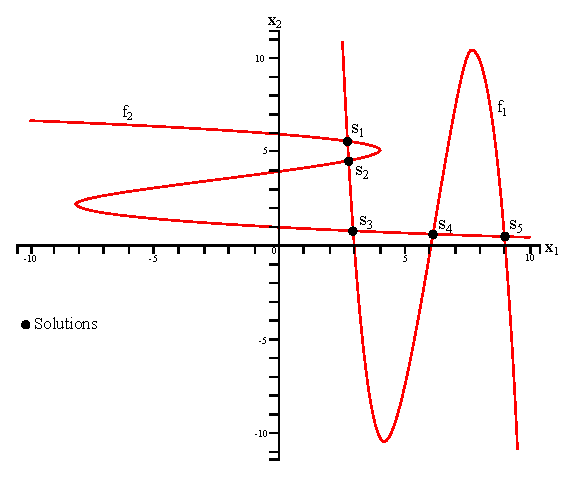
\includegraphics[scale=0.8]{chap3/figs/doblelimit_mul_1.eps}
\caption{Five solution system.}
\label{9sol}
\end{figure}

The proposed Homotopy formulation is:

\begin{displaymath}
\begin{array}{c}
H_1(f_1,\lambda)=\lambda(\lambda+1)(\lambda-1)(\lambda-2)(x_1-13)(x_1+13)+(\lambda-0.5)^2 f_1^2=0\\
H_2(f_2,\lambda)=\lambda(\lambda+1)(\lambda-1)(\lambda-2)(x_2-13)(x_2+13)+(\lambda-0.5)^2 f_2^2=0\\
\end{array}
\end{displaymath}

where the solution line es placed at $\lambda=0$ and $\lambda=1$. For practical purposes, just the symmetrical branch for the Homotopy path linked to solution line $\lambda=1$ is plotted.

Initial point is chosen as $A=[x_1=-13,x_2=-13]$ and tracing of the path is started, resulting in a global convergence to all the solutions of the system ($S_1,S_2,S_3,S_4$ and $S_5$) (see figure \ref{homotex}). Final point is $B=[x_1=13, x_2=13]$ and the Homotopy path for each variable ($x_1-\lambda$ and $x_2-\lambda$) are shown in figures \ref{fig:subfig:xxx1} and \ref{fig:subfig:xxx2}.

\begin{figure}[hbtp]
\centering
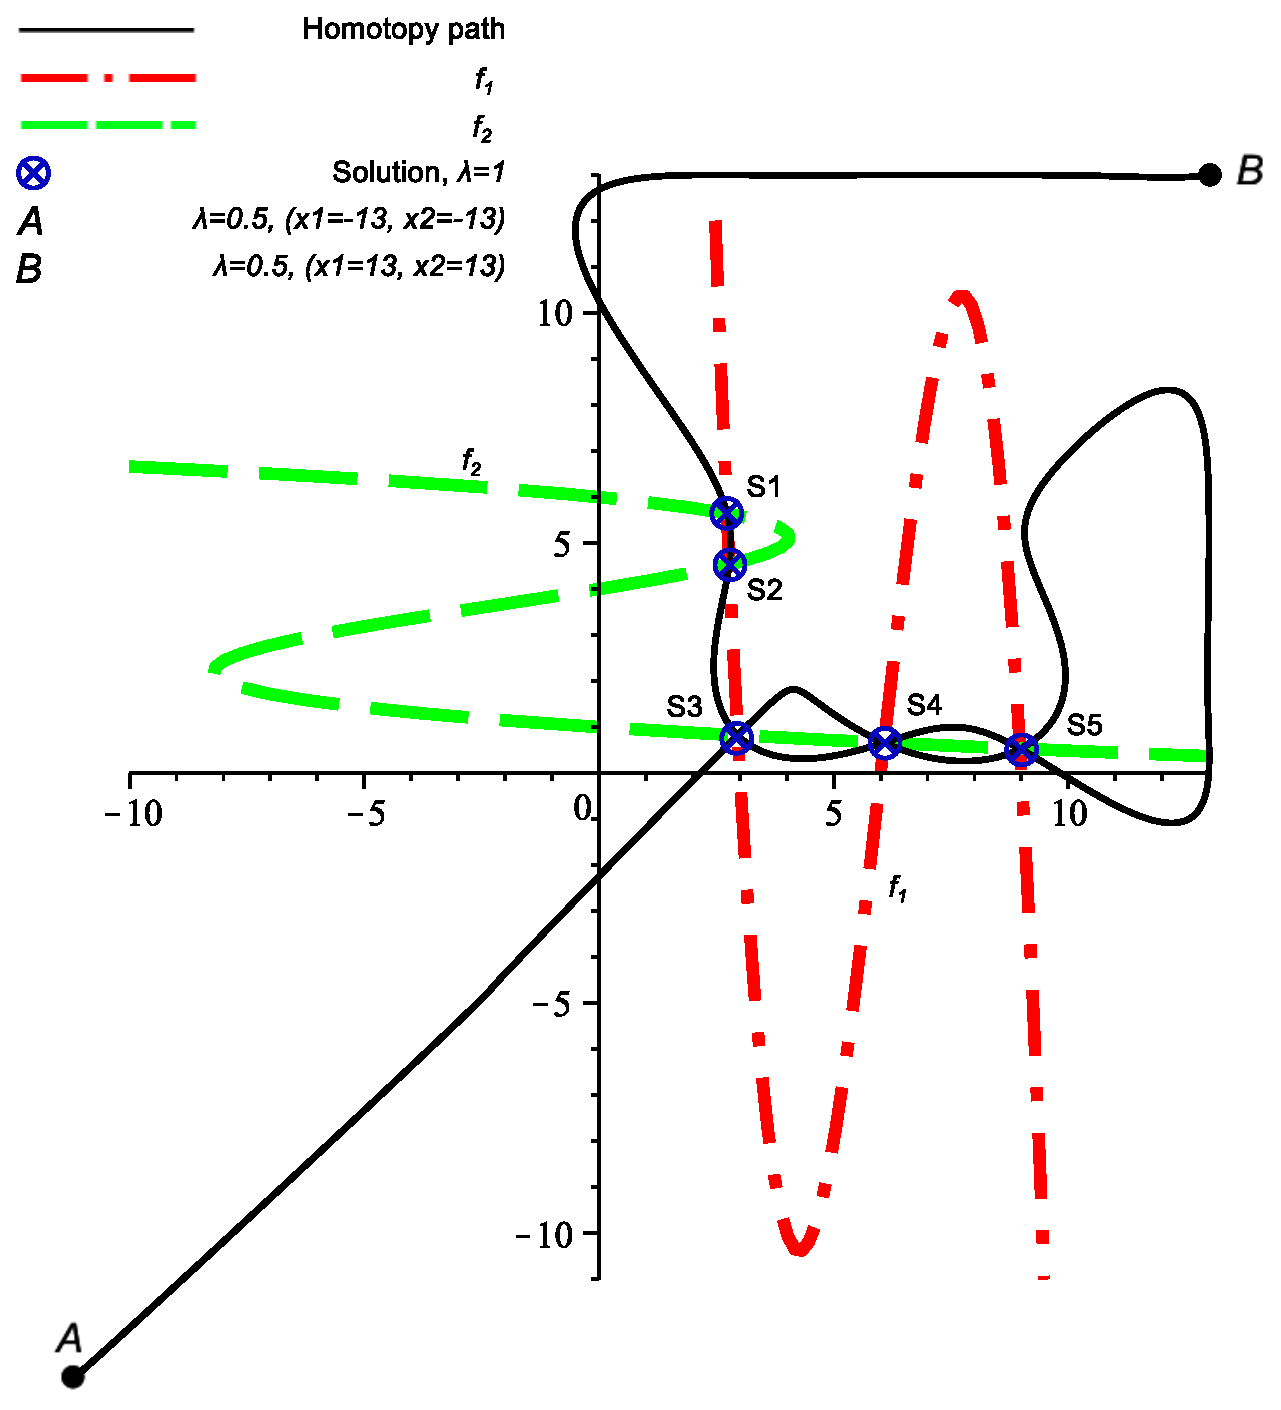
\includegraphics[scale=0.5]{ejem4lim/POLINOM4LIMA.eps}
\caption{Homotopy path for the 2 variable example.}
\label{homotex}
\end{figure}

\begin{figure}[hbtp]
\begin{center}
%% --- first subfigure ---
\subfloat[Homotopy path $\lambda$-$x_1$]{
	\label{fig:subfig:xxx1}
	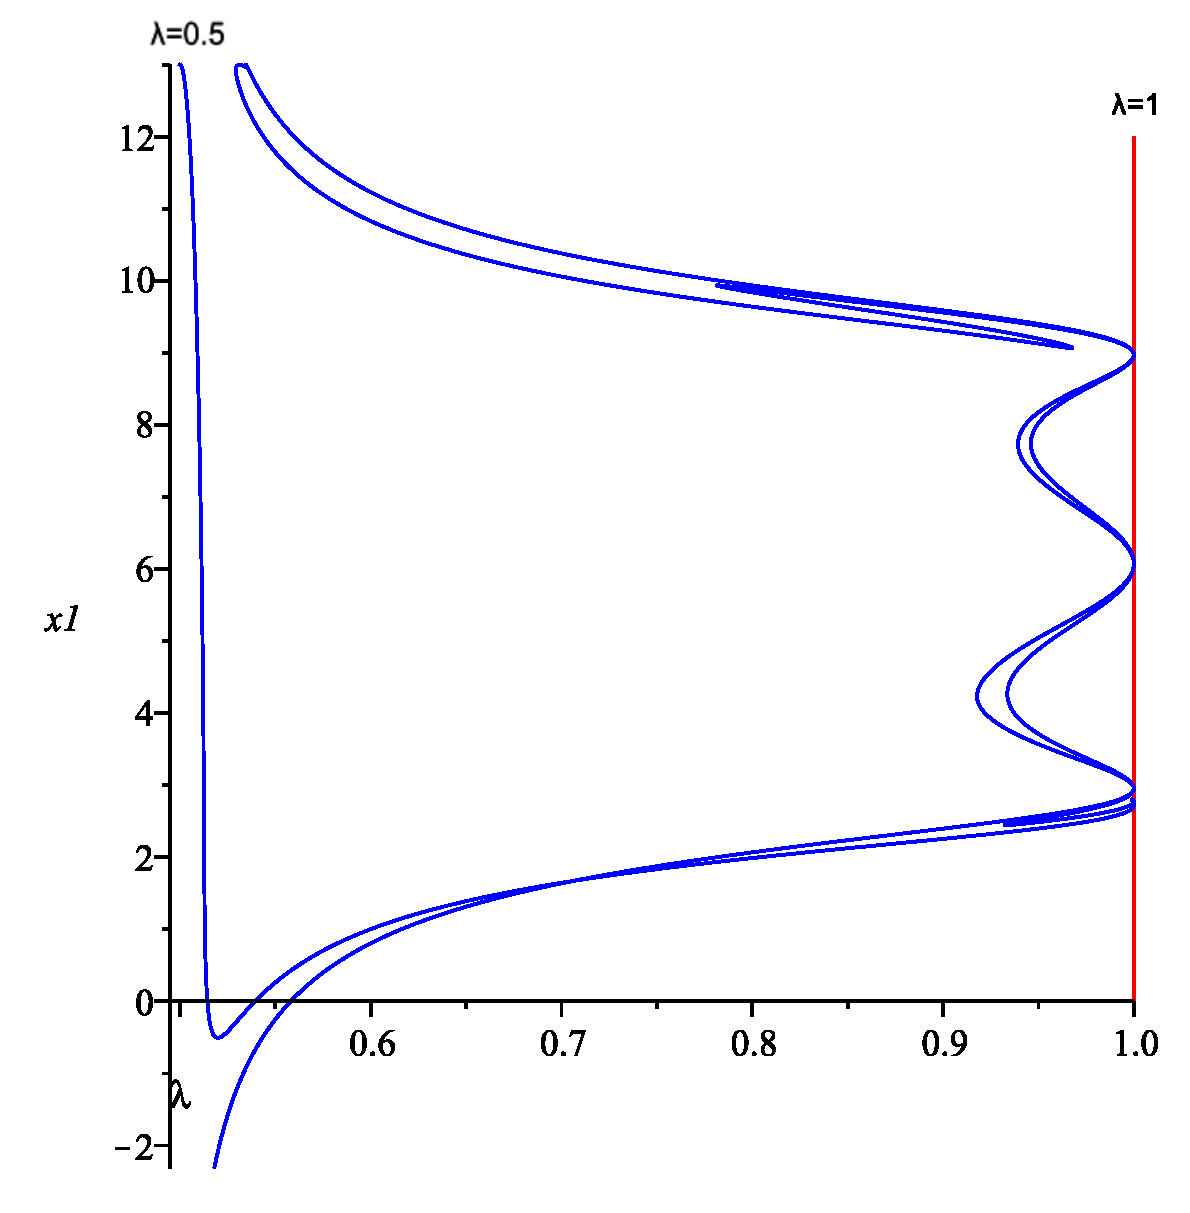
\includegraphics[scale=0.4]{ejem4lim/POLINOM4LIMAx1.eps}}
%% --- second subfigure ---
\subfloat[Homotopy path $\lambda$-$x_2$]{
	\label{fig:subfig:xxx2}
	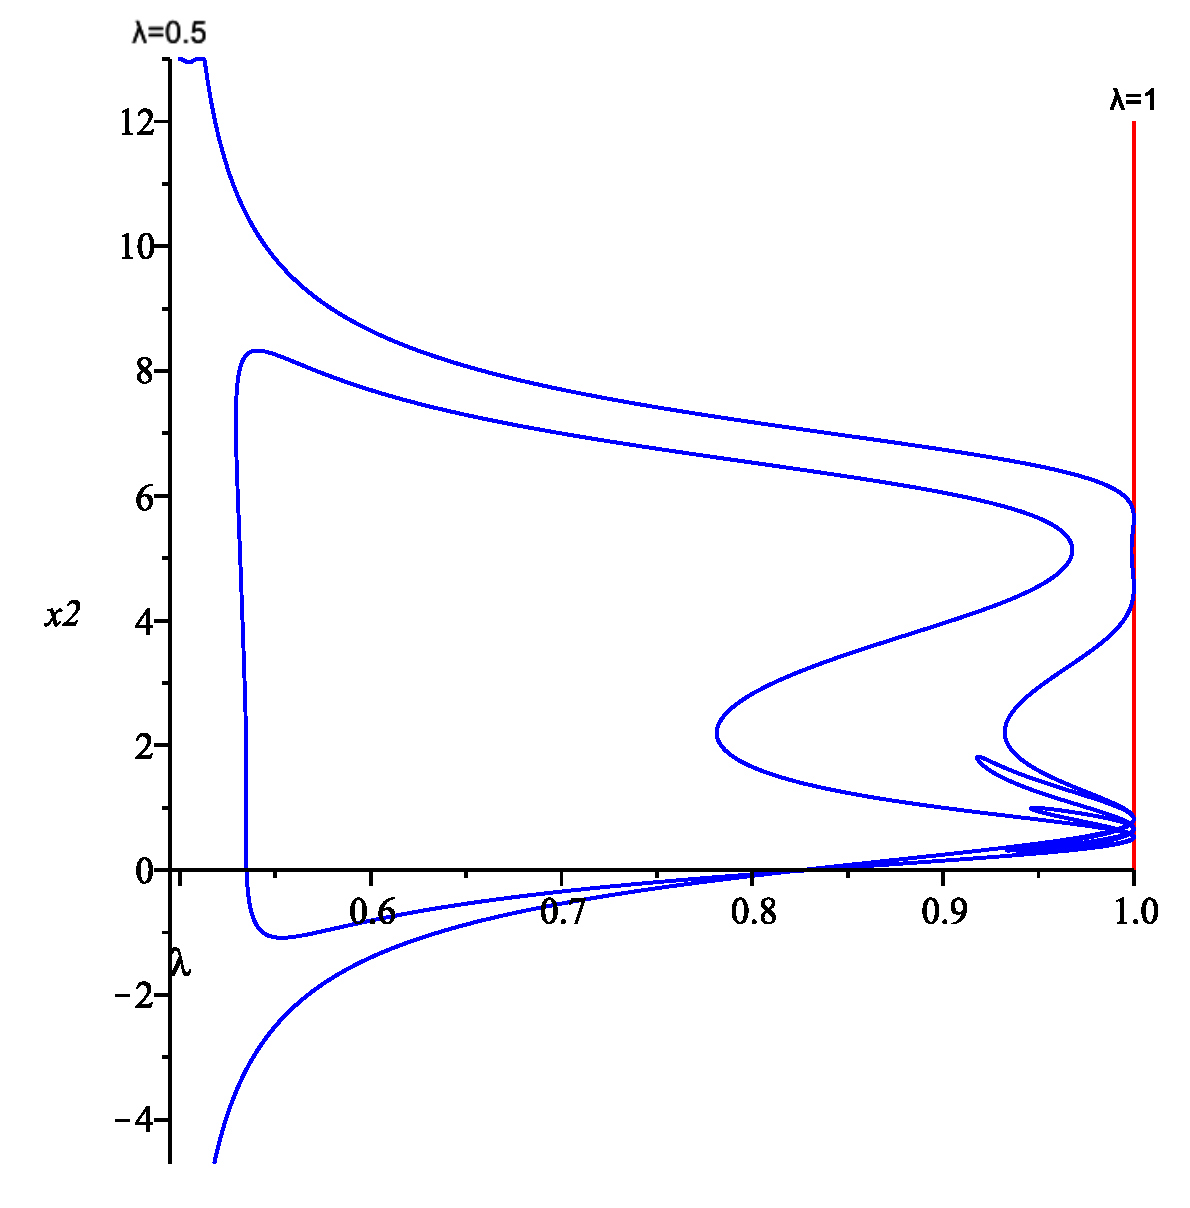
\includegraphics[scale=0.4]{ejem4lim/POLINOM4LIMAx2.eps}}
\end{center}
\caption{Homotopy paths.}
\label{fig:subfig}
\end{figure}

\subsection{Circuit with two tunnel diodes}

Tunnel diodes have non-linear behavior, which can be depicted in general way in figure \ref{fig:subfig1:tunelmod}. As it can be seen, tunnel diode has three sign changes on the slope which combined with a load line could produce up to three solutions per tunnel diode present in the circuit. In this example, the model chosen for the tunnel diode is a function of exponential terms \cite{homo_sze},\cite{homo_shur} and can be expressed as:

\begin{displaymath}
i=I_p({V \over V_p})e^{1-{V \over V_p}}+I_0e^{{q \over {KT}} V}
\end{displaymath}

Exponential terms can produce numerical overflows, thus this circuit represents a challenge for the double bounded Homotopy. Hence, in this example an ERDD circuit is presented; consists of 2 tunnel diodes, a voltage source, and a resistor all of them connected in series (see figure \ref{fig:subfig1:2tunel}). The voltage source $V_1$ has the value $1V$ and the resistor $R_2$ is $20\Omega$. Besides, both tunnel diodes ($K_3$ and $K_4$) have the same model with coefficients:
$Ip=100 \times 10^{-3}$,
$V_p=50 \times 10^{-3} $, $I_0=1\times 10^{-9}$ y ${q \over {KT}} = 40$. The equilibrium equation is formulated form the modified nodal analysis of the circuit. Besides, the system is reduced to three equations eliminating the nodal voltage $v_1$ because its constant and equal to the voltage source value. Therefore, variables taken into account are: $I_E$, $v_2$, and $v_3$. Equations are expressed as:

\begin{displaymath}
\begin{array}{l}
f_1=  {1 \over 20}-{v_2 \over 20}+I_E =0\\ \\
f_2=  -{1 \over 20}+{v_2 \over 20}+2(v_2-v_3)e^{(1-20v_2+20v_3)} \\+1\times 10^{-9}e^{(40v_2-40v_3)} =0 \\\\
f_3=  2(v_2-v_3)e^{(1-20v_2+20v_3)}+1\times 10^{-9}e^{(40v_2-40v_3)} \\ 
-2v_3e^{(1-20v_3)}-1\times 10^{-9} e^{(40v_3)} =0
\end{array}
\end{displaymath}

\begin{figure}[hbtp]
\begin{center}
%% --- first subfigure ---
\subfloat[Model for tunnel diode.]{
	\label{fig:subfig1:tunelmod}
	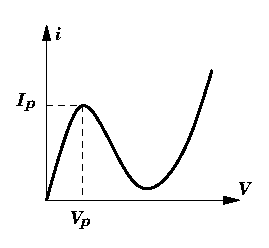
\includegraphics[scale=1.3]{chap4/figs/tunnelmod.eps}}
\hspace{0.5in}
%% -- second subfigure ---
\subfloat[Circuit with two tunnel diodes.]{
	\label{fig:subfig1:2tunel} 
	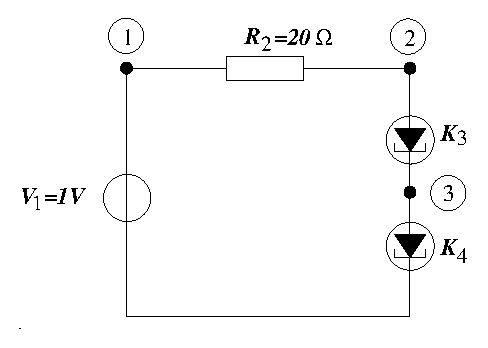
\includegraphics[scale=0.85]{chap4/figs/erdd.eps}}
\end{center}
\caption{Tunnel diode study case.}
\label{fig:subfig1}
\end{figure}

Now, DBH is applied to solve the circuit, the Homotopy formulation is expressed as follows:

\begin{displaymath}
\begin{array}{c}
H_1(f_1,\lambda)=\lambda(\lambda+1)(\lambda-1)(\lambda-2)(I_E-1)(I_E+1)+(\lambda-0.5)^2 f_1^2=0\\
H_2(f_2,\lambda)=\lambda(\lambda+1)(\lambda-1)(\lambda-2)(v_2-1)(v_2+1)+(\lambda-0.5)^2 f_2^2=0\\
H_3(f_3,\lambda)=\lambda(\lambda+1)(\lambda-1)(\lambda-2)(v_3-1)(v_3+1)+(\lambda-0.5)^2 f_3^2=0\\
\end{array}
\end{displaymath}

where bounding lines are $a=0$ and $b=1$, and initial point for the Homotopy path is selected at $A=[I_E=-1,v_2=-1,v_3=-1]$.

As result for the Homotopy tracing all the operating points were located, 9 points in total. Also, the final point for the path is located at $B=[I_E=1,v_2=1,v_3=1$. Figure \ref{2tunelg}(b) shows a close-up to the solutions region, here can be seen how the path crosses through the 9 solutions, presenting 3 sub-regions ($F1$, $F2$ y $F3$). In order to observe in detail the behavior of the path, an enlargement for each one of the regions $F1$, $F2$, and $F3$ is also shown (see
figuras \ref{2tunelg}(c), \ref{2tunelg}(d), and \ref{2tunelg}(e)). In these figures all 9 solutions ($S_1, S_2, S_3, S_4, S_5, S_6, S_7, S_8$ y $S_9$) are shown on the Homotopy path.

\begin{figure}[hbtp]
\psfrag{L}{$\lambda$}
\centering
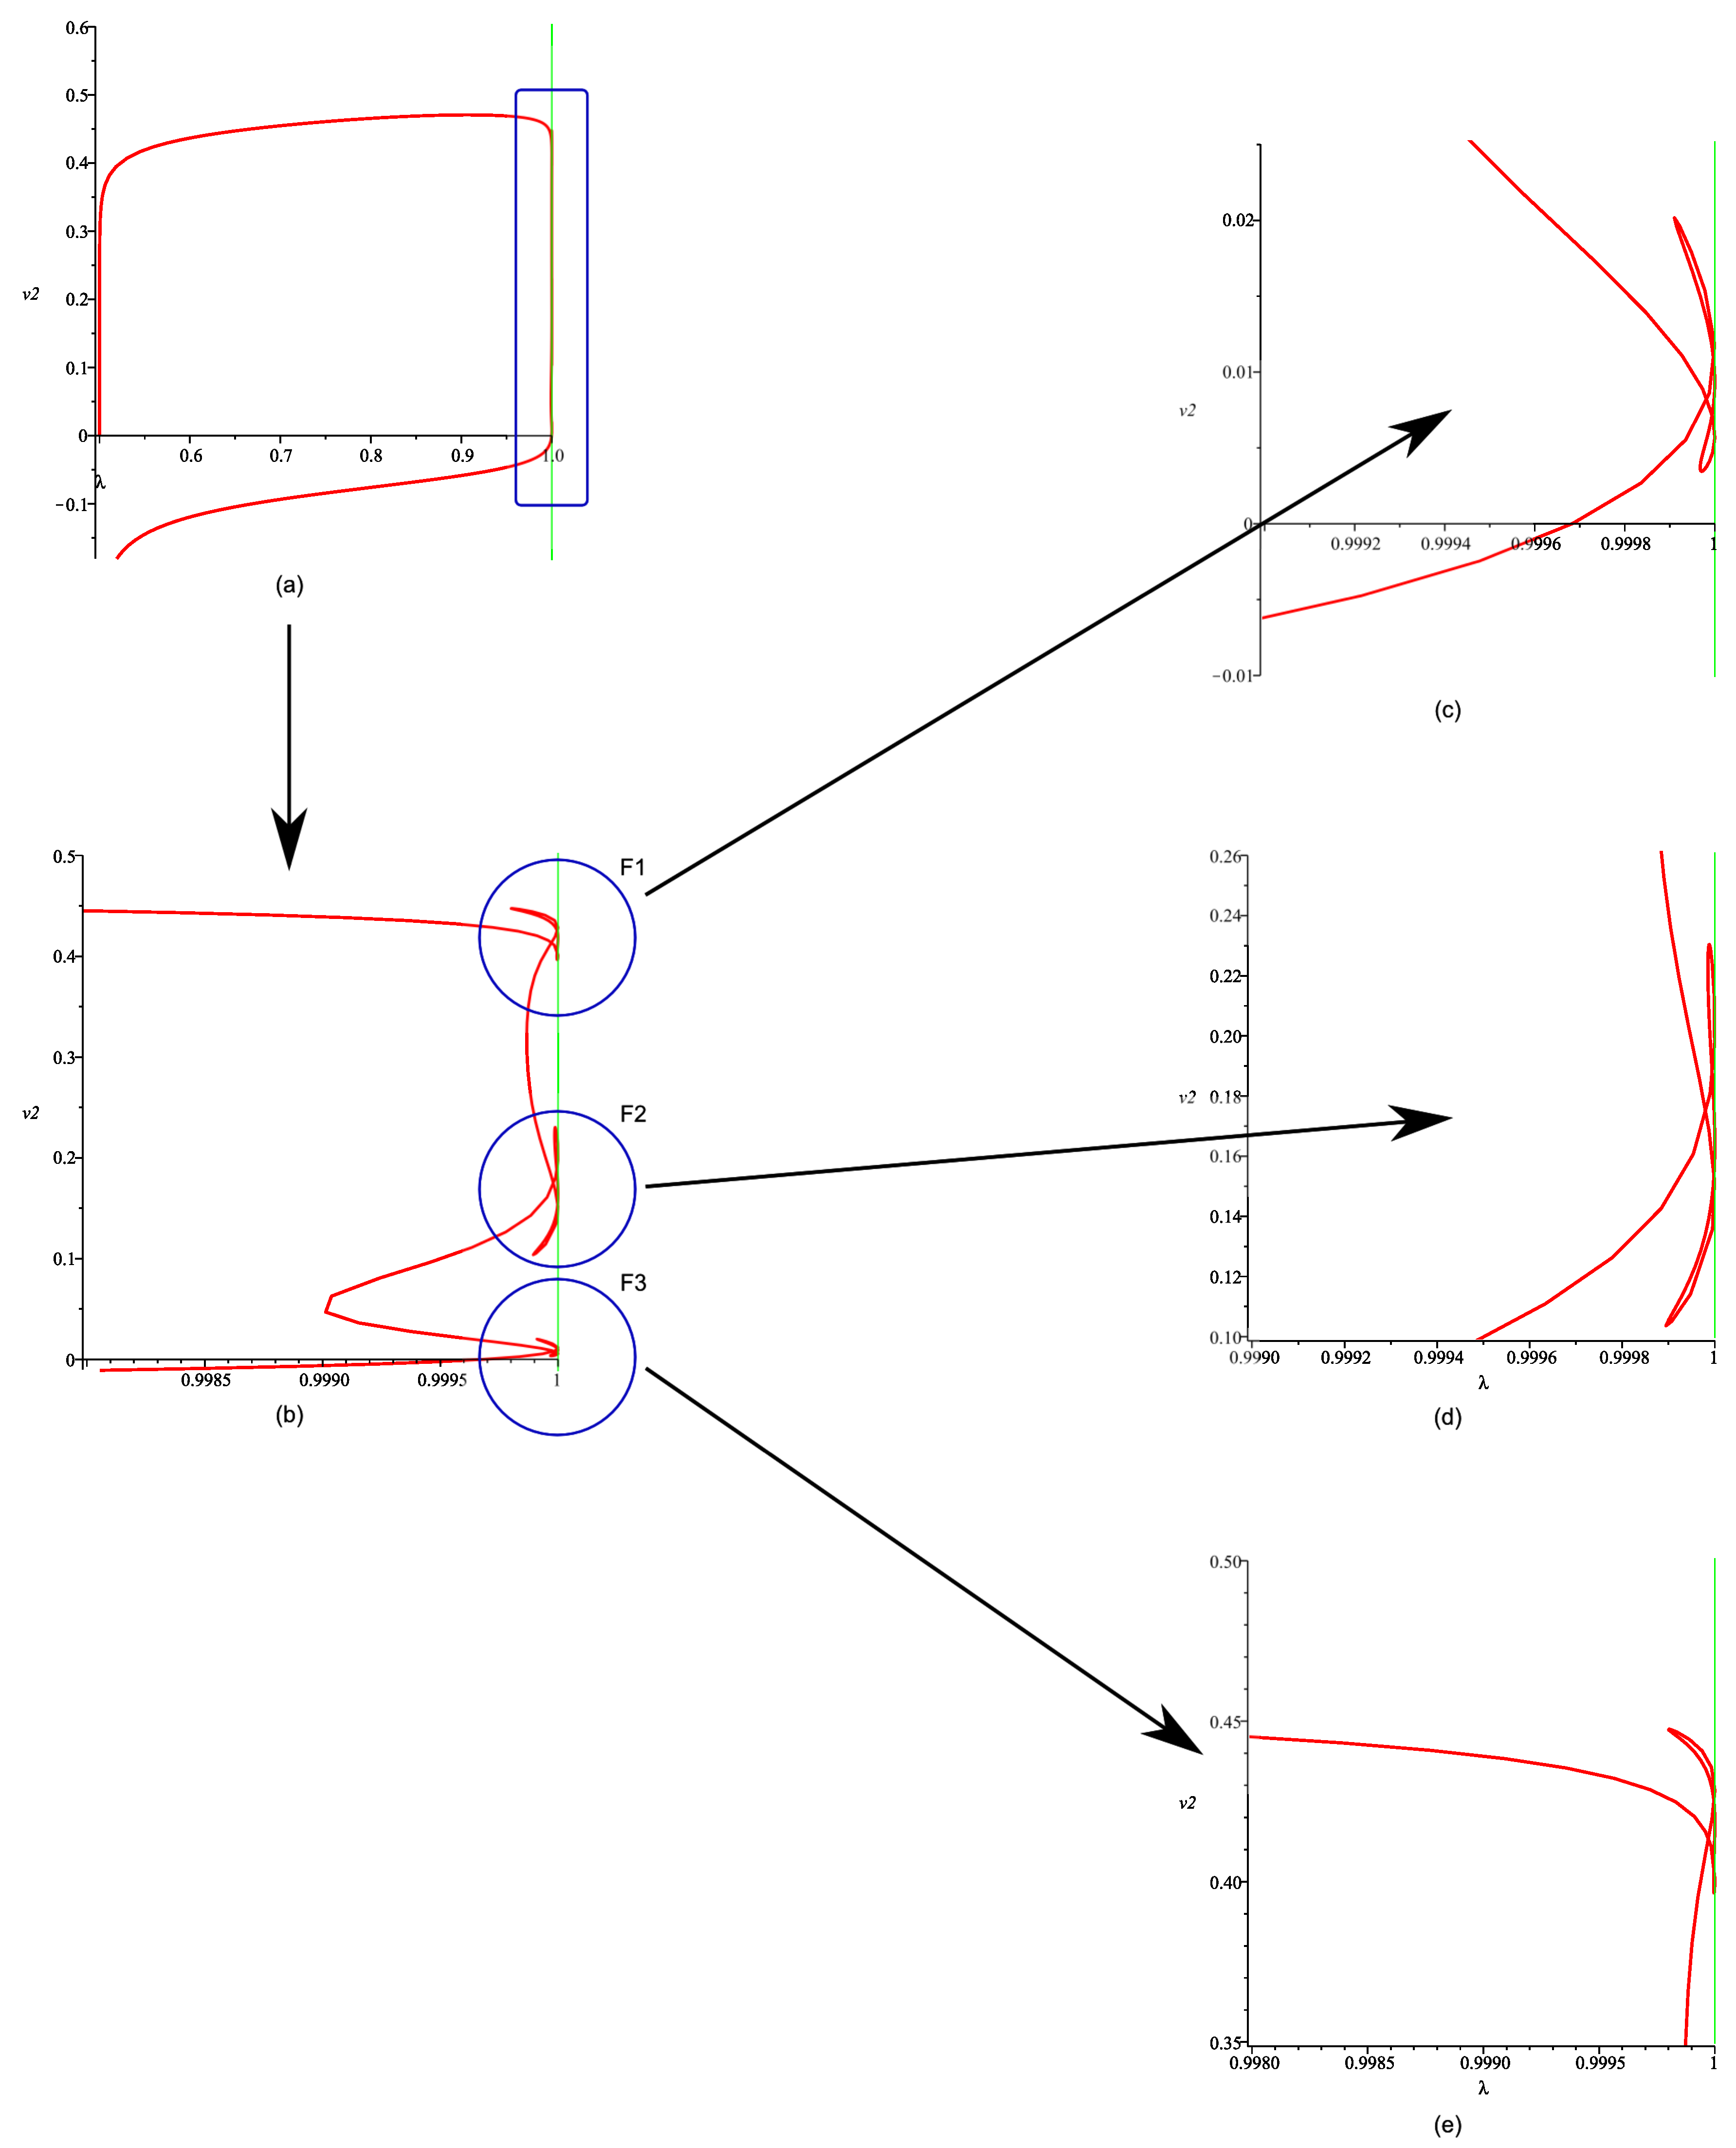
\includegraphics[scale=0.25]{ejem4lim/TUNEL_COMPLETE.eps}
\caption{Homotopy path for the circuit with tunnel diodes.}
\label{2tunelg}
\end{figure}

\subsection{Circuit with bipolar transistors and a diode}

A circuit with bipolar transistors and a diode was reported in \cite{homo_tadeusiewicz} and  \cite{homo_yamamurawise}, it was solved using piecewise methods. Then, in \cite{homo_yamamura}, the circuit was resolved using modified fixed point Homotopy. This circuit has 3 operating points. The Ebers-Moll is used for all the transistors. The equation for the model is given as:

\begin{displaymath}
\left[ \begin{array}{c}
i_{D_E} \\
i_{D_C}
\end{array}\right] =
\left[ \begin{array}{cc} 1  & \alpha_R \\
\alpha_F & 1 \\
\end{array}\right] \left[ \begin{array}{c}
10^{-9}(e^{(40v_{be})} - 1) \\
10^{-9}(e^{(40v_{bc})} - 1)
\end{array}\right]
\end{displaymath}

The circuital rendering of the model is shown in figure \ref{FEbersMoll}.

As for the diode, the model is:

\begin{displaymath}
i_d=10^{-9}(e^{40u} - 1)
\end{displaymath}

\begin{figure*}[tbp]
\centerline{
\epsfxsize=110mm
\epsffile{chap4/figs/diotran.eps}
}
\caption{Circuit with bipolar transistors and a diode.}
\label{yamamuracircuito}
\end{figure*}

\begin{figure}[hbtp]
\psfrag{f}{$\alpha_F$}
\psfrag{r}{$\alpha_R$}
\centerline{
\epsfxsize=36mm
\epsffile{chap4/figs/ebersmoll.eps}}
\caption{Ebers-Moll model for bipolar transistor.}
\label{FEbersMoll}
\end{figure}

The values for the circuit components can be found in table \ref{yamamuracircuitovalores}. First, the equilibrium equation is formulated using the modified nodal analysis with the result of a system having 14 equations and 14 variables. The circuit is shown in figure \ref{yamamuracircuito} and the equilibrium equation es \ref{eqsd} (using MNA circuital analysis).

\begin{table}[hbtp]
\center{
{\scriptsize
\begin{tabular}{||c|c||}
\hline\hline
Component  & Value  \\ \hline\hline
$R_1$ & $4K\Omega$   \\ \hline
$R_2$ & $0.1K\Omega$   \\ \hline
$R_3$ & $8K\Omega$   \\ \hline
$R_4$ & $8K\Omega$   \\ \hline
$R_5$ & $4K\Omega$   \\ \hline
$R_6$ & $0.1K\Omega$   \\ \hline
$R_7$ & $30K\Omega$   \\ \hline
$R_8$ & $1K\Omega$   \\ \hline
$R_9$ & $0.1K\Omega$   \\ \hline
$R_{10}$ & $10K\Omega$   \\ \hline
$R_{11}$ & $4K\Omega$   \\ \hline
$R_{12}$ & $10K\Omega$   \\ \hline
$R_{13}$ & $1K\Omega$   \\ \hline
$V_{cc}$ & $12V$   \\ \hline  \hline
\end{tabular}
}
}
\caption{Circuit components and values.}
\label{yamamuracircuitovalores}
\end{table}

{\tiny
\begin{equation}
\begin{array}{|r||r|} 
f_1 & {\frac {37}{20000}}\,{\it v_1}-{\frac {1}{4000}}\,{\it v_2}-{\frac {1}{
 4000}}\,{\it v_6}-{\frac {1}{1000}}\,{\it v_9}-{\frac {1}{4000}}\,{\it 
v_{12}}-{\frac {1}{10000}}\,{\it v_{13}}+{\it IE}=0 \\  
f_2 & -{\frac {1}{4000}}\,{\it v_1}+{\frac {3}{8000}}\,{\it v_2}-{\frac {1}{
8000}}\,{\it v_5}+ 0.00000000990\,{{\rm e}^{40\,{\it v_4}-40\,{\it v_3}}}
+ 0.00000000010- 0.000000010\,{{\rm e}^{40\,{\it v_4}-40\,{\it v_2}}}=0  \\  
f_3 & {\frac {1}{100}}\,{\it v_3}- 0.000000010\,{{\rm e}^{40\,{\it v_4}-40\,{
\it v_3}}}+ 0.00000000990+ 0.00000000010\,{{\rm e}^{40\,{\it v_4}-40\,{
\it v_2}}}=0 \\
f_4 & {\frac {1}{8000}}\,{\it v_4}-{\frac {1}{8000}}\,{\it v_6}+ 0.00000000010
\,{{\rm e}^{40\,{\it v_4}-40\,{\it v_3}}}- 0.00000001000+ 0.00000000990
\,{{\rm e}^{40\,{\it v_4}-40\,{\it v_2}}}=0 \\
f_5 & -{\frac {1}{8000}}\,{\it v_2}+{\frac {1}{8000}}\,{\it v_5}+
 0.00000000010\,{{\rm e}^{40\,{\it v_5}-40\,{\it v_7}}}- 0.00000001000+
 0.00000000990\,{{\rm e}^{40\,{\it v_5}-40\,{\it v_6}}}=0 \\
f_6 & -{\frac {1}{4000}}\,{\it v_1}-{\frac {1}{8000}}\,{\it v_4}+{\frac {3}{
8000}}\,{\it v_6}+ 0.00000000990\,{{\rm e}^{40\,{\it v_5}-40\,{\it v_7}}}
+ 0.00000001010- 0.000000010\,{{\rm e}^{40\,{\it v_5}-40\,{\it v_6}}}-
 0.000000010\,{{\rm e}^{40\,{\it v_8}-40\,{\it v_6}}}=0 \\
f_7 & {\frac {1}{100}}\,{\it v_7}- 0.000000010\,{{\rm e}^{40\,{\it v_5}-40\,{
\it v_7}}}+ 0.00000000990+ 0.00000000010\,{{\rm e}^{40\,{\it v_5}-40\,{
\it v_6}}}=0 \\
f_8 & {\frac {1}{30000}}\,{\it v_8}-{\frac {1}{30000}}\,{\it v_9}+ 0.000000010
\,{{\rm e}^{40\,{\it v_8}-40\,{\it v_6}}}- 0.000000010=0 \\
f_9 & -{\frac {1}{1000}}\,{\it v_1}-{\frac {1}{30000}}\,{\it v_8}+{\frac {31}{
30000}}\,{\it v_9}+ 0.00000000990\,{{\rm e}^{40\,{\it v_{11}}-40\,{\it v_{10}
}}}+ 0.00000000010- 0.000000010\,{{\rm e}^{40\,{\it v_{11}}-40\,{\it v_9}}
}=0 \\
f_{10} & {\frac {1}{100}}\,{\it v_{10}}- 0.000000010\,{{\rm e}^{40\,{\it v_{11}}-40\,
{\it v_{10}}}}+ 0.00000000990+ 0.00000000010\,{{\rm e}^{40\,{\it v_{11}}-40
\,{\it v_9}}}=0 \\
f_{11} & {\frac {1}{10000}}\,{\it v_{11}}-{\frac {1}{10000}}\,{\it v_{12}}+
 0.00000000010\,{{\rm e}^{40\,{\it v_{11}}-40\,{\it v_{10}}}}- 0.00000001000
+ 0.00000000990\,{{\rm e}^{40\,{\it v_{11}}-40\,{\it v_9}}}=0 \\
f_{12} & -{\frac {1}{4000}}\,{\it v_1}-{\frac {1}{10000}}\,{\it v_{11}}+{\frac {7}{
20000}}\,{\it v_{12}}+ 0.00000000990\,{{\rm e}^{40\,{\it v_{13}}}}+
 0.00000000010- 0.000000010\,{{\rm e}^{40\,{\it v_{13}}-40\,{\it v_{12}}}}=0 \\
f_{13} & -{\frac {1}{10000}}\,{\it v_1}+{\frac {11}{10000}}\,{\it v_{13}}+
 0.00000000010\,{{\rm e}^{40\,{\it v_{13}}}}- 0.00000001000+
 0.00000000990\,{{\rm e}^{40\,{\it v_{13}}-40\,{\it v_{12}}}}=0 \\
 f_{14} & v_1-12=0 \\
\end{array}
\label{eqsd}
\end{equation}}

Now, DBH is applied to solve the circuit; the Homotopy formulation is expressed as follows:

\begin{displaymath}
\begin{array}{c}
H_1(f_1,\lambda)=\lambda(\lambda+1)(\lambda-1)(\lambda-2)(v_1-13)(v_1+13)+C(\lambda-0.5)^2 f_1^2=0\\
H_2(f_2,\lambda)=\lambda(\lambda+1)(\lambda-1)(\lambda-2)(v_2-13)(v_2+13)+C(\lambda-0.5)^2 f_2^2=0\\
\vdots \\
H_{14}(f_{14},\lambda)=\lambda(\lambda+1)(\lambda-1)(\lambda-2)(I_E-13)(I_E+13)+C(\lambda-0.5)^2 f_{14}^2=0\\
\end{array}
\end{displaymath}

where the constant value $C=0.000001$, the bounding lines are $a=0$ and $b=1$, and the initial point for the Homotopy path is selected as shown in table \ref{iniyama}.

\begin{table}[tbp]
{\small
\center{
\hspace{-4mm}
\begin{tabular}{||c|c|c|c|c|c|c|c|c|c|c|c|c|c|c||}
\hline\hline
Point & $v_1$ & $v_2$ & $v_3$ & $v_4$ & $v_5$ & $v_6$ & $v_7$ & $v_8$ & $v_9$ & $v_{10}$& $v_{11}$ & $v_{12}$ & $v_{13}$ & $i_E$ \\ \hline
Initial &  +13 & -13 & +13 & -13 & -13 & -13 & -13 & -13 & -13 & -13 & -13 & -13 & -13 & -13  \\ \hline
Final &  +13 & +13 & +13 & +13 & -13 & +13 & -13 & +13 & +13 & +13 & +13 & +13 & +13 & +13  \\ \hline
\end{tabular}
}
}
\caption{Initial point and final point.}
\label{iniyama}
\end{table}

So, the next step is to solve the circuit using the double bounded Homotopy, resulting in the convergence to the three known solutions for the circuit. The Homotopy path correspondent to the current of the voltage source $I_E$ is displayed in figure \ref{yamaie}. Finally, the final point for the Homotopy trace is exhibited in table \ref{iniyama}.

\begin{table*}[tbp]
{\small
\center{
\hspace{-4mm}
\begin{tabular}{||c|c|c|c|c|c|c|c|c|c|c|c|c|c|c||}
\hline\hline
Sol & $v_1$ & $v_2$ & $v_3$ & $v_4$ & $v_5$ & $v_6$ & $v_7$ & $v_8$ & $v_9$ & $v_{10}$& $v_{11}$ & $v_{12}$ & $v_{13}$ & $i_E$ \\ \hline
$S_1$ &  12 & 5.995 & 0.085 &0.368 &0.712 &0.436 &0.390 &0.699 &11.635 &0.4e-5 &0.039 &0.039 &0.321 &-0.0089 \\ \hline
$S_2$ & 12 & 0.883 & 0.278 &0.590 &0.631 &0.812 &0.315 &1.074 &11.647 &0.4e-5 &0.039 &0.039 &0.321 &-0.0100 \\ \hline
$S_3$ & 12 & 0.405 & 0.366 &0.685 &0.349 &6.796 &0.070 &7.038 &11.839 &0.4e-5 &0.039 &0.039 &0.321 &-0.0085 \\ \hline \hline
\end{tabular}
}
}
\caption{Solutions for the circuit with bipolar transistors and a diode.}
\label{yamamuracircuitosoluc}
\end{table*}

\begin{figure}
\centering
\begin{minipage}[c]{0.5\linewidth}
	\centering
	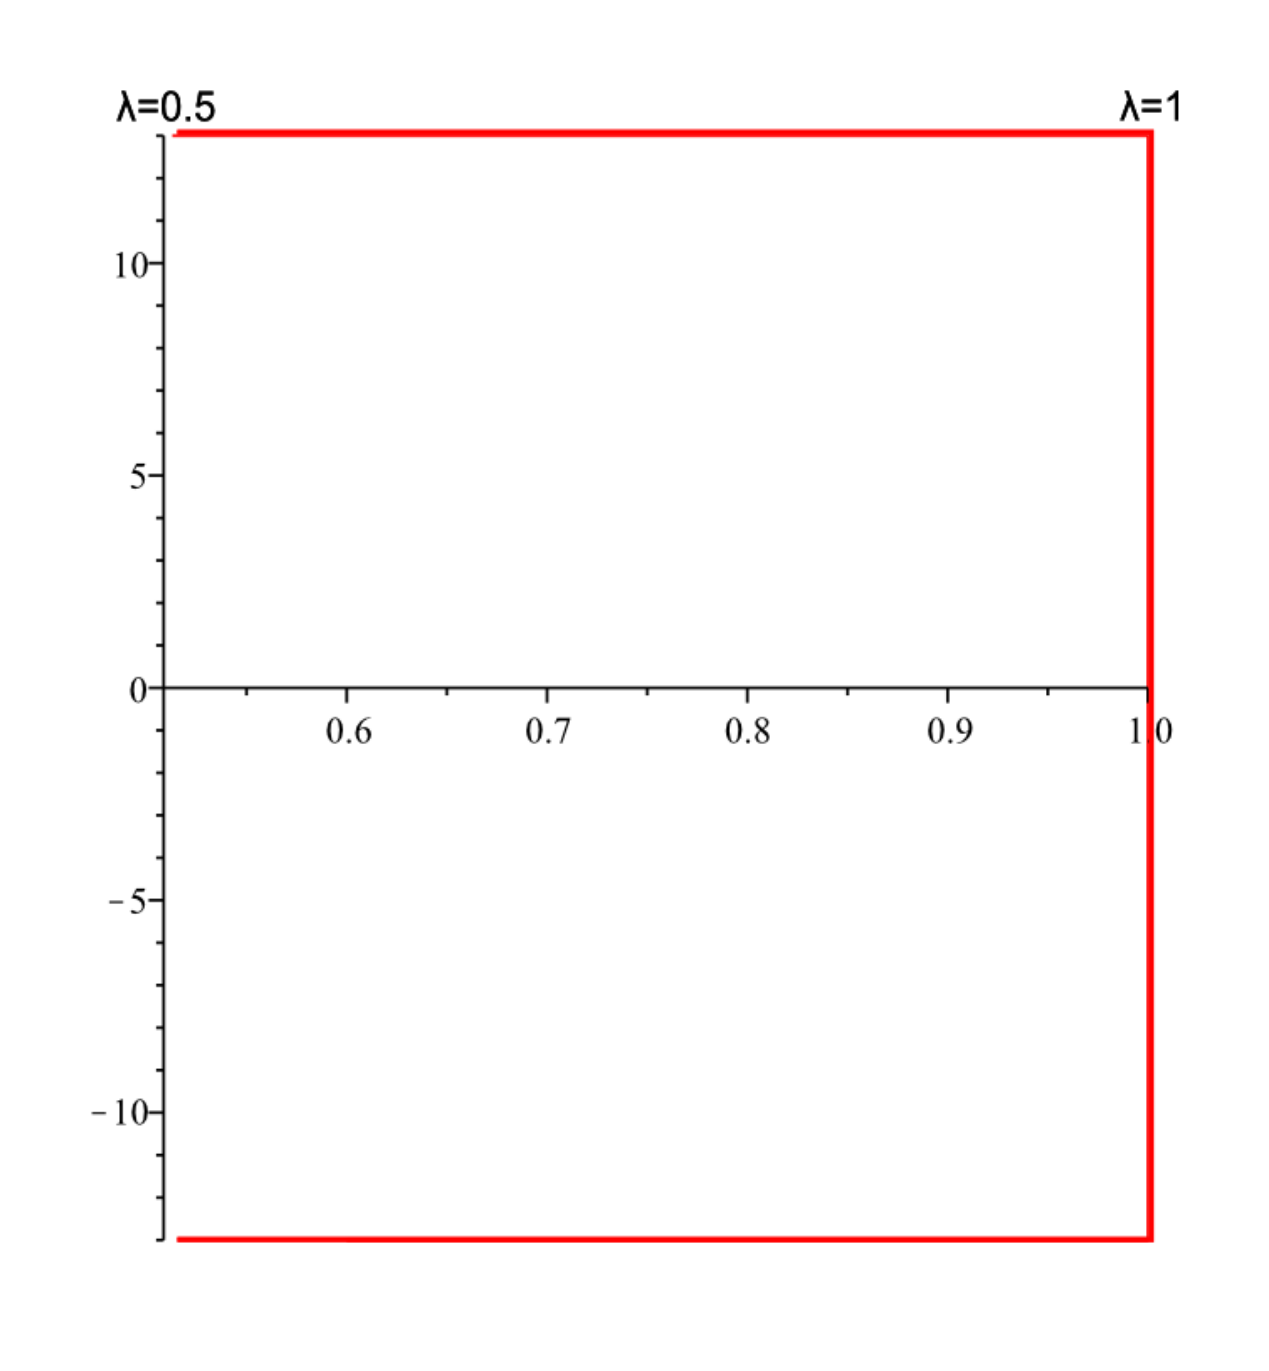
\includegraphics[scale=0.3]{ejem4lim/YAMAMURAV8A.eps}
\end{minipage}%
\hspace{-0.05in}
\begin{minipage}[c]{0.5\linewidth}
	\centering
	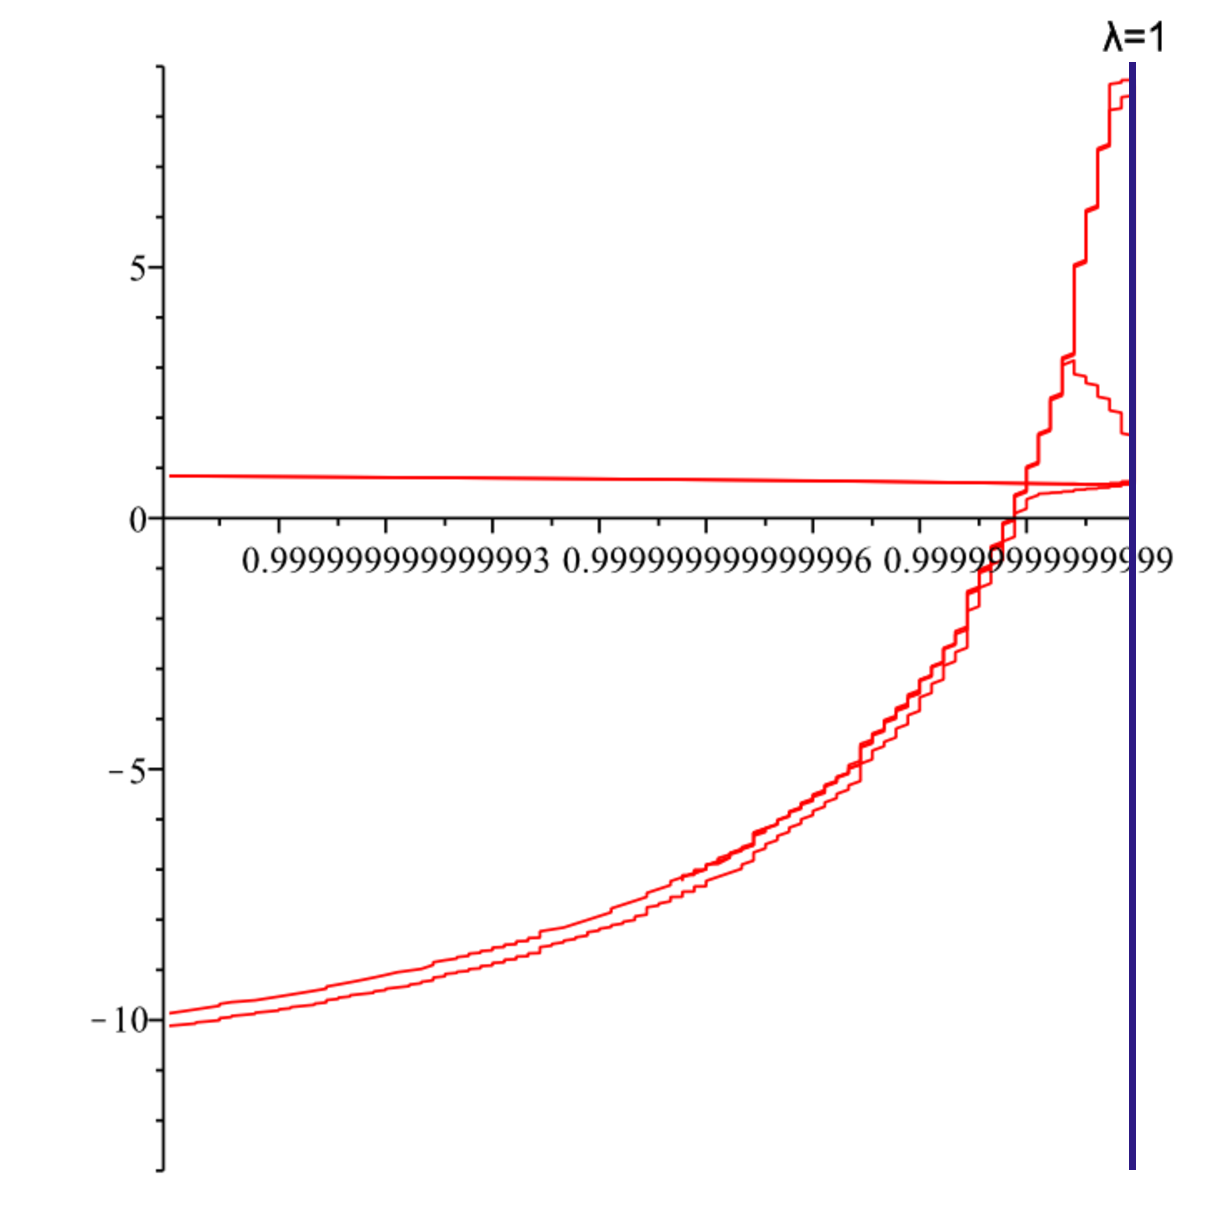
\includegraphics[scale=0.3]{ejem4lim/YAMAMURAV8.eps}
\end{minipage}
\caption{Homotopy path $\lambda-v_8$.}
\label{yamaie}
\end{figure}


\subsection{Chua's Circuit}

Chua's circuit \cite{homo_chua} (see figura \ref{chua}), with 9 solutions, has become in the reference circuit for Homotopy applied to circuit analysis. The values for the components are shown in table \ref{chuatablet}. This circuit has 4 bipolar transistors modeled by the Ebers-Moll model for the bipolar transistor operating in the direct active region (see figure \ref{eber}).

\begin{table}[hbtp]
\center{
{\scriptsize
\begin{tabular}{||c|c|c|c||}
\hline\hline
Component  & Value  & Component & Value\\ \hline\hline
$R_1$ & $1k\Omega$ & $R_9$ & $10.1k\Omega$    \\ \hline
$R_2$ & $4k\Omega$ & $R_{10}$ & $10.1k\Omega$  \\ \hline
$R_3$ & $4k\Omega$  &  $R_{11}$ & $4k\Omega$  \\ \hline
$R_4$ & $5k\Omega$  &  $R_{12}$ & $4k\Omega$  \\ \hline
$R_5$ &  $30k\Omega$ & $R_{13}$ & $30k\Omega$    \\ \hline
$R_6$  & $0.5k\Omega$ & $R_{14}$ & $30k\Omega$  \\ \hline
$R_7$ & $0.5k\Omega$  &  $V_1$ & $10V$  \\ \hline
$R_8$ & $30k\Omega$  &  $V_2$ & $2V$  \\ \hline
$V_{CC}$ & $12V$  &  $\alpha$& $0.98$     \\ \hline\hline
\end{tabular}
}
}
\caption{Component values for Chua's circuit.}
\label{chuatablet}
\end{table}

\begin{figure}[hbtp]
\centerline{
\epsfxsize=70mm
\epsffile{chap4/figs/chua.eps}}
\caption{Chua's circuit with 9 solutions.}
\label{chua}
\end{figure}


\begin{figure}[hbtp]
\psfrag{F}{{\tiny $I_D=10^{-9}(e^{40v_D}-1)$}}
\psfrag{b}{{\tiny $\alpha=0.98$}}
\centerline{
\epsfxsize=35mm
\epsffile{chap4/figs/eber.eps}}
\caption{Half-side Ebers-Moll model.}
\label{eber}
\end{figure}

The resulting equation system is:

\begin{displaymath}
{\small
\begin{array}{l}
f_1=4.3663v_2+0.6103168 \times 10^{-5} e^{(40v_1)}-12\\+0.2863168\times 10^{-5}e^{(40v_2)}=0 \\ \\
f_2=5.4v_1+v_3+0.3580\times 10^{-5}e^{(40v_1)}-22\\+7\times 10^{-7}e^{(40v_3)}+  5\times 10^{-7}e^{(40v_4)}+0.6620\times 10^{-5}e^{(40v_2)}=0 \\ \\
f_3=4.3663v_4+0.6103168\times 10^{-5}e^{(40v_3)}-12\\+0.2863168\times 10^{-5}e^{(40v_4)}=0 \\
\end{array}
}
\end{displaymath}

Now, the DBH is applied to solve the circuit. The Homotopy formulation is expressed as:

\begin{displaymath}
\begin{array}{c}
H_1(f_1,\lambda)=\lambda(\lambda+1)(\lambda-1)(\lambda-2)(v_1-10)(v_1+10)+(\lambda-0.5)^2 f_1^2=0\\
H_2(f_2,\lambda)=\lambda(\lambda+1)(\lambda-1)(\lambda-2)(v_2-10)(v_2+10)+(\lambda-0.5)^2 f_2^2=0\\
H_3(f_3,\lambda)=\lambda(\lambda+1)(\lambda-1)(\lambda-2)(v_3-10)(v_3+10)+(\lambda-0.5)^2 f_3^2=0\\
H_4(f_4,\lambda)=\lambda(\lambda+1)(\lambda-1)(\lambda-2)(v_4-10)(v_4+10)+(\lambda-0.5)^2 f_3^2=0\\
\end{array}
\end{displaymath}

where the bounding lines are $a=0$ and $b=1$, and the initial point for the Homotopy path es selected at $A=[v_1=10,v_2=10,v_3=10,v_4=10]$.

Equilibrium equation is the same as employed in \cite{homo_chua}. The variables to be solved are branch voltages: $v_1$, $v_2$, $v_3$, and $v_4$. Figure \ref{chuaf} shows the Homotopy path for the branch voltage $v_1$. The final point for the path was $B=[v_1=-10,v_2=10,v_3=10,v_4=10]$. Finally, the Homotopy was able to find 2 out of 9 solutions. The remaining 7 roots were isolated in one or more separate paths.

\begin{figure}[hbtp]
\centerline{
\epsfxsize=60mm
\epsffile{ejem4lim/CHUA1V1.eps}
\epsfxsize=60mm
\epsffile{ejem4lim/CHUA2V1.eps}
}
\caption{Chua's circuit solution.}
\label{chuaf}
\end{figure}

Found solutions are:

\begin{displaymath}
\begin{array}{r}
\left[\begin{array}{r}
v_1 \\ v_2  \\ v_3  \\ v_4  \\
\end{array}\right]
\begin{array}{r}
 \\ = \\ \\ \end{array}
\underbrace{\left[\begin{array}{r}
0.3300 \\ 0.3680 \\ 0.3367 \\ 0.3642 \\
\end{array}\right]}_{\mbox{Solution \ding{172}}},
\underbrace{\left[\begin{array}{r}
 -0.7119 \\ 0.3775 \\ 0.3350 \\ 0.3653 \\
\end{array}\right]}_{\mbox{Solution \ding{173}}},
\end{array}
\end{displaymath}

\section{Conclusions}

The stop criterion for Homotopy methods consist in using a maximum number (arbitrarily number) of integration steps, in such a way that when integration steps reach the solution line the algorithm stops. Nevertheless, this kind of method may leave some roots out. A set of properties fo the PDA4 Homotopy were explained and developed. The bounded Homotopy with four solution lines shows interesting properties given by the fact that allows the Homotopy path to be placed between two limits named bounding lines. Also, the curvature radius on the solutions shows a proportional relationship with the separation between solution lines. Additionally, the curvature radius on the turning points of the solutions spatially matches with the critical points of the equilibrium equation and is directly proportional to $f(x)$ evaluated at the return. Another fundamental property of this new Homotopy is to possess a symmetry axis, which is found between solution lines ($\lambda=0$ and $\lambda=a$), allowing the implementation for a stop criterion. Finally, bounded Homotopy with 4 solution lines was applied to DC simulations for some circuit examples and to a mathematical example, showing its potential to be used on non-linear circuit analysis.

\bibliographystyle{amsplain}
\bibliography{nuevah2}

\end{document}


